\documentclass[tikz, border=10pt]{standalone}
\usepackage{pgfplots}
\usepgfplotslibrary{groupplots}
\pgfplotsset{compat=1.18}

\begin{document}
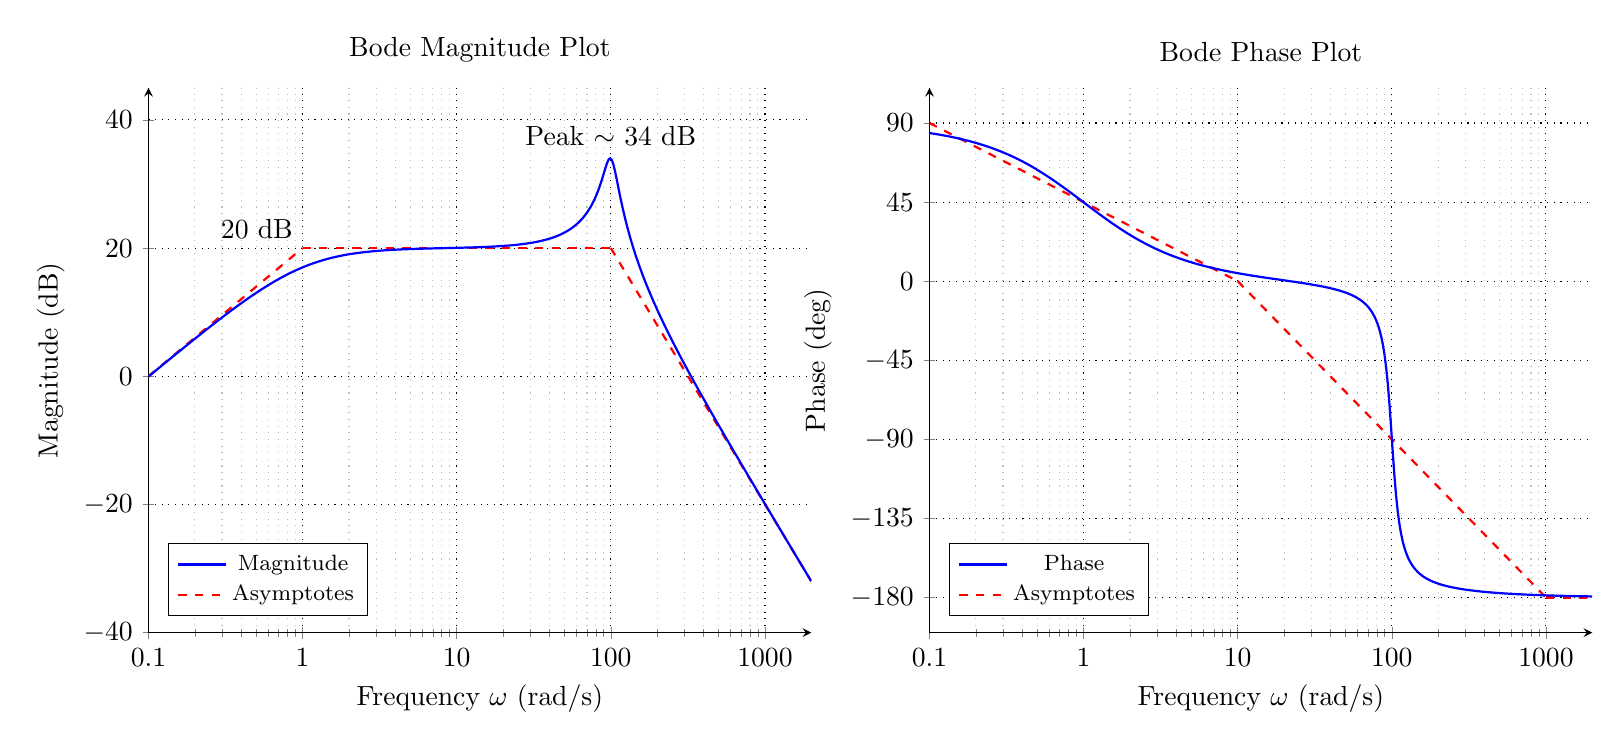
\begin{tikzpicture}
    \begin{groupplot}[
        group style={
            group size=2 by 1,
            horizontal sep=1.5cm,
        },
        width=10cm, height=8.5cm,
        xlabel={Frequency $\omega$ (rad/s)},
        xmin=0.1, xmax=2000,
        xmode=log,
        grid=both,
        major grid style={dotted, black},
        minor grid style={dotted, gray!50},
        axis lines=left,
        xtick={0.1, 1, 10, 100, 1000},
        xticklabels={$0.1$, $1$, $10$, $100$, $1000$},
    ]

    % Magnitude Plot
    \nextgroupplot[
        ylabel={Magnitude (dB)},
        ymin=-40, ymax=45,
        legend pos=south west,
        legend style={font=\footnotesize},
        title={Bode Magnitude Plot}
    ]
    % Asymptotes Magnitude
    \draw[thick, red, dashed] (axis cs: 0.1, 0) -- (axis cs: 1, 20);
    \draw[thick, red, dashed] (axis cs: 1, 20) -- (axis cs: 100, 20);
    \draw[thick, red, dashed] (axis cs: 100, 20) -- (axis cs: 2000, -32);
    
    % Actual Curve
    \addplot[thick, blue, domain=0.1:2000, samples=400] {20*log10( 10*x / ( sqrt(1+x^2) * sqrt( (1-(x/100)^2)^2 + (0.002*x)^2 ) ) )};
    
    \addlegendentry{Magnitude}
    \addlegendimage{thick, red, dashed}
    \addlegendentry{Asymptotes}

    % Annotations
    \node[anchor=south east] at (axis cs: 1, 20) {20 dB};
    \node[anchor=south] at (axis cs: 100, 34.5) {Peak $\sim$ 34 dB};

    % Phase Plot
    \nextgroupplot[
        ylabel={Phase (deg)},
        ymin=-200, ymax=110,
        ytick={-180, -135, -90, -45, 0, 45, 90},
        legend pos=south west,
        legend style={font=\footnotesize},
        title={Bode Phase Plot}
    ]
    
    % Asymptotes Phase
    \draw[thick, red, dashed] (axis cs: 0.1, 90) -- (axis cs: 0.1, 90); % start
    \draw[thick, red, dashed] (axis cs: 0.1, 90) -- (axis cs: 10, 0);
    \draw[thick, red, dashed] (axis cs: 10, 0) -- (axis cs: 1000, -180);
    \draw[thick, red, dashed] (axis cs: 1000, -180) -- (axis cs: 2000, -180);

    % Actual Curve Phase
    \addplot[thick, blue, domain=0.1:2000, samples=400] {90 - atan(x) - atan2(0.002*x, 1-(x/100)^2)};

    \addlegendentry{Phase}
    \addlegendimage{thick, red, dashed}
    \addlegendentry{Asymptotes}

    \end{groupplot}
\end{tikzpicture}
\end{document}
